\paragraph{Data efficiency (RQ4).}
Training on 10\,\%, 25\,\%, 50\,\% and 100\,\% of the training split gives macro-F1 \lcNoneTen{}, \lcNoneTwentyFive{}, \lcNoneFifty{}, \lcNoneFull{} for the plain model and
\lcAcgTen{}, \lcAcgTwentyFive{}, \lcAcgFifty{}, \lcAcgFull{} for ACG-ConvNeXt (Fig.~\ref{fig:lc}). The curves overlap: guidance does not help more when data are scarce.
\begin{figure}[t]
\centering
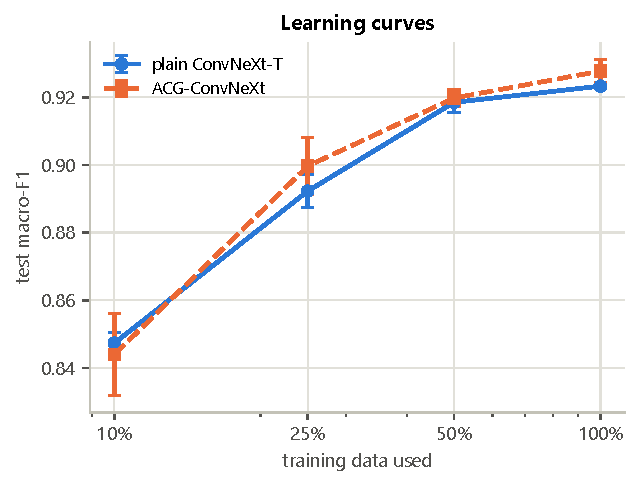
\includegraphics[width=0.8\columnwidth]{learning_curves.pdf}
\caption{Learning curves (mean $\pm$ SD over 3 seeds).}
\label{fig:lc}
\end{figure}

\paragraph{Learning-rate sensitivity.}
Deep hyper-parameters were not tuned per variant. For seed 0, the plain model scores \lrNoneHalf{}, \lrNoneDef{} and \lrNoneDouble{} at half, default and double learning rate, and the guided model \lrAcgHalf{}, \lrAcgDef{} and \lrAcgDouble{}:
changing the learning rate moves macro-F1 by as much as any ablation effect, and the default rate was evidently not optimal for the plain model.
The guided model's seed-0 score at the doubled rate looked like a clear gain, but that rate was singled out after seeing test results, so we replicated it as an exploratory, post hoc check with three seeds per variant:
plain \lrTwoPlain{}\,$\pm$\,\lrTwoPlainSD{}, guided \lrTwoAcg{}\,$\pm$\,\lrTwoAcgSD{} ($\Delta=$ \lrTwoDelta{}, 95\,\% CI \lrTwoLo{} to \lrTwoHi{}, unadjusted bootstrap $p=$ \lrTwoP{}).
Both variants improve over the default rate and the gap between them is not distinguishable from zero, so the null conclusion holds at the better learning rate as well. A fully fair comparison would tune every variant on validation data, which we did not do.

\paragraph{Robustness.}
On \robN{} stratified test frames, JPEG compression at quality 50 lowers accuracy from \robPlainClean{} to \robPlainJpegFifty{} for the plain model, but only from \robAcgClean{} to \robAcgJpegFifty{} for the guided model (Fig.~\ref{fig:rob}).
At quality 10 the figures are \robPlainJpegTen{} against \robAcgJpegTen{}, and under Gaussian blur with $\sigma=3$\,px \robPlainBlurThree{} against \robAcgBlurThree{}.
\emph{The controls reproduce this advantage:} shuffled-image contours give \robShufJpegFifty{} and the central ellipse \robEllJpegFifty{} at quality 50, and global features alone give \robGfeatJpegFifty{}.
Robustness therefore comes from supplying colour and texture statistics computed on the pixels, not from the contour's alignment with the lesion.
\begin{figure*}[t]
\centering
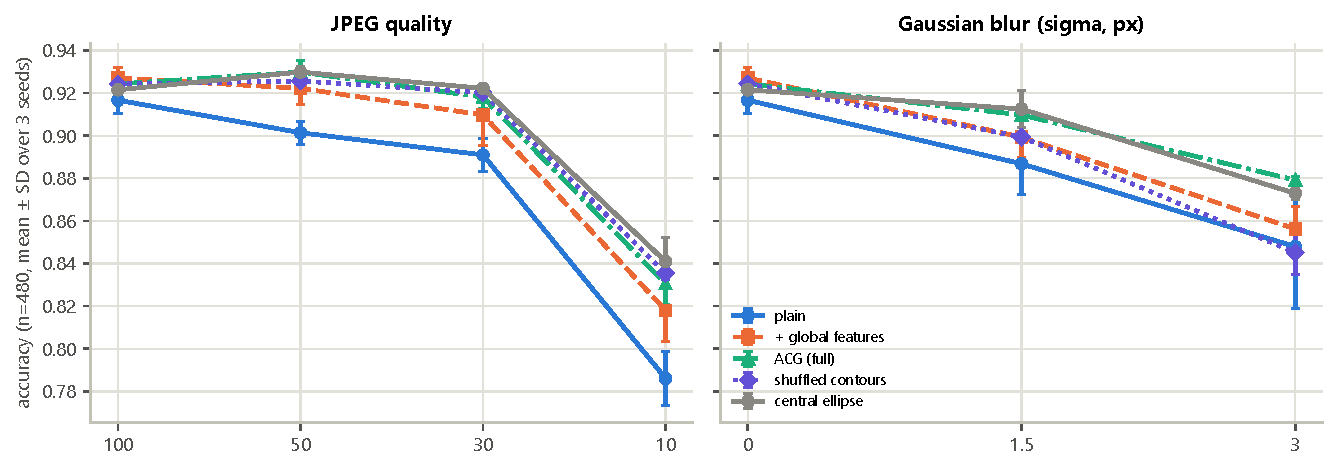
\includegraphics[width=0.7\textwidth]{robustness_multiseed.pdf}
\caption{Accuracy under JPEG compression and Gaussian blur (mean $\pm$ SD over 3 seeds, 480 test frames; contours and features recomputed on the degraded pixels).}
\label{fig:rob}
\end{figure*}

\paragraph{Interpretability.}
\emph{Grad-CAM against expert masks.} Using the polyp-class Grad-CAM on the 176 Kvasir-SEG test-split polyps, the CAM maximum lies inside the expert mask for \plainPoint{} of frames for the plain model and \acgPoint{} for the guided model;
the top-20\,\% CAM pixels overlap the mask with IoU \plainCamIoU{} and \acgCamIoU{}. The CAM maximum falls inside the active contour for \plainCamInAC{} and \acgCamInAC{} of frames.
With $n=176$ these differences are within sampling noise: the guided network does not attend to lesions more accurately than the plain one.
\emph{TreeSHAP} on LightGBM with global and contour features attributes \shapRegion{} of the total importance to inside/outside colour and texture (region) features and \shapGlobal{} to global features, but only \shapShape{} to contour shape and \shapBoundary{} to boundary features:
the geometry of the contour carries little information.
\emph{Layer-wise linear probes} on ConvNeXt-T stages give macro-F1 \lwPreOne{} (pretrained) and \lwFtOne{} (fine-tuned) at stage~1, \lwPreThree{} and \lwFtThree{} at stage~3, and \lwPreFour{} and \lwFtFour{} at stage~4:
fine-tuning mostly reshapes the last two stages.

